% !TeX root = ../main.tex

\chapter{算法测试与结果}

\section{复现SVRG}

为保证对论文\inlinecite{johnsonAcceleratingStochasticGradient}的理解正确以及不遗漏技术细节,这里本文使用Julia编程语言复现了论文中对SVRG与SGD的性能测试。

所有测试中损失函数表达式均为
\begin{equation}\label{key}
P(w) = \frac1n \sum_{i=1}^n f_i(w)
\end{equation}
$f_i(w)$为随机生成的$w$的二次型,保证论文中强凸条件以及莱布尼兹连续条件被满足。$w$维度为6.

\begin{figure}[htb]
	\centering
	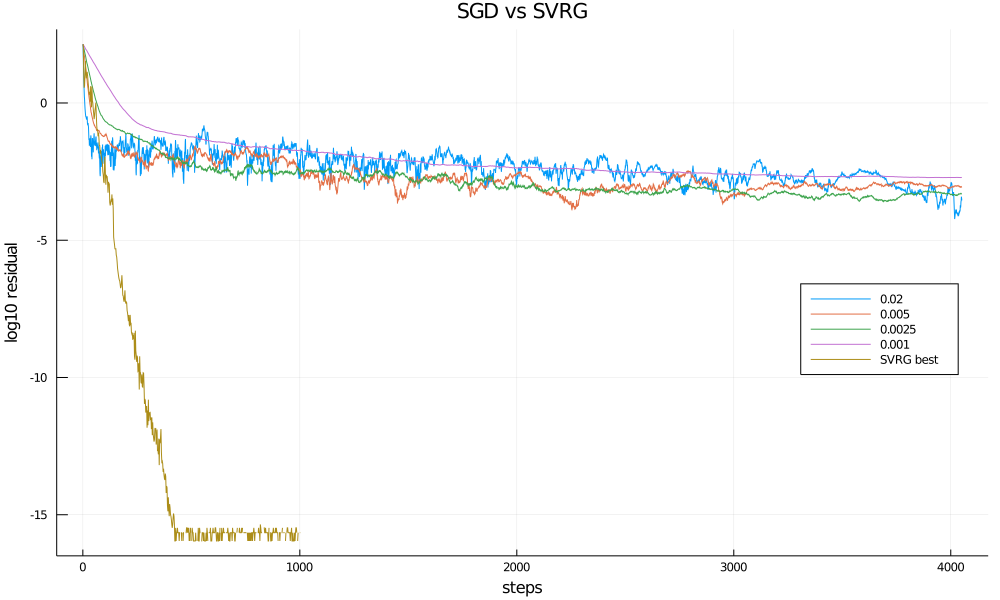
\includegraphics[width=1\textwidth]{image/sgd-vs-svrg.pdf}
	\caption{SGD与SVRG性能测试}
	\label{fig:sgd-svrg}
	\note{注:图中复现了论文中的算法性能比较\cite[7]{johnsonAcceleratingStochasticGradient},图例中前4条为SGD在最优学习速率附近不同值处的表现,最后一条为SVRG接近最优参数下的一个结果,数字表示步长(学习速率)。图中对SVRG数据的横坐标进行了$\frac{m+n}{m}$的拉伸,保证相同横坐标下使用的数据集数量相等。}
\end{figure}
\begin{figure}[htb]
	\centering
	\includegraphics[width=1\textwidth]{image/sgd-vs-svrg2.pdf}
	\caption{SGD、SVRG与GD性能测试}
	\label{fig:sgd-svrg2}
	\note{注:接上图,加入了与常用无随机性梯度下降(GD)的比较,其横坐标被扩大$n$倍以保证相同横坐标数据量相等}
\end{figure}

在图\ref{fig:sgd-svrg}中SVRG的表现远优于基础的SGD算法,且与论文中测试结果一致。

